\section{Results and Discussion}
\label{sec:results}
We report the final per-run values of each metric, aggregated over up to $n=10$
runs per configuration (Table~\ref{tab:results}). Because several outcomes are
bounded counts with (near-)zero variance---for which the assumptions of a
parametric $t$-test do not hold---group comparisons use distribution-free tests
(Mann--Whitney $U$, whose $p$ is computed by case: the \emph{exact} $U$
distribution for untied samples with $n_1+n_2\le20$ (all pairs here), a
two-sided exact permutation $p$ for fully separated constant arms, and the
tie-corrected normal approximation only when ties are present), reported with the
Cliff's $\delta$ effect size and $95\%$ bootstrap confidence intervals, with
numeric $p$-values Holm-corrected across the confirmatory family; equivalence is
assessed by a two one-sided test (TOST) and per-mission success by Wilson-score
intervals.
Runs in which the platform did not move
(travelled distance $\approx 0$) are a startup-reliability
outcome rather than a navigation result: of the $160$ attempted runs, $154$ met the
movement criterion for behavioral analysis and $6$ remained immobile. The
observable, published criterion for these six is \emph{immobility} (the analyzer's
distance criterion; most carry an accumulated mission clock but no motion); we read
them as consistent with an \emph{initialization} failure (the navigation container
not bringing the robot up), rather than the mid-mission timeouts of the earlier
submission, but do not certify that infrastructure cause from published raw logs. We report two complementary views rather than pooling them:
(i) performance \emph{conditional on successful initialization}, computed on the
valid runs ($n=8$--$10$ per configuration); and (ii) \emph{per-attempt} startup
reliability ($154/160=96.25\%$). We do \emph{not} average the immobile runs into
the behavioral metrics---their zero distance and zero inspection would bias the
means and rates---but report them separately as the reliability outcome; the
per-run values (with per-run seeds and outcomes) are released with the code.
%% R2#4: "the boundary between confirmatory and exploratory claims is not always
%% easy to trace through the narrative". Declaracao explicita da familia, e cada
%% alegacao no texto passa a dizer de qual familia vem.
\paragraph*{Confirmatory and exploratory claims} We fix the boundary here and mark it
at every claim rather than only in the tables. The \emph{confirmatory} family,
specified before the new runs were executed, contains three comparisons in the
scenarios they were designed for: the proposed layer against the generic heuristic
and against the one-factor selection variant in the \texttt{default} scenario, and
the keep-out-only ablation against the fixed patrol carrying the same keep-out
(KOa vs.\ KOF) on the on-route hazard. Those are Holm-corrected within the family and
are reported with $p_{\mathrm{Holm}}$. Everything else---the \texttt{conflict} and
\texttt{adverse} scenarios, the threshold and hysteresis sweeps, the marginal-hazard
configuration, and every re-analysis of previously recorded runs---is
\emph{exploratory}, is reported with uncorrected $p$, and is labelled as exploratory
in the sentence that states it. Two of the analyses below are additionally
\emph{retrospective}: the confirmation-distance re-scoring and the boundary-crossing
count operate on runs recorded for the earlier submission, and are planned now rather
than in advance.

The principal (confirmatory) comparisons are consolidated in
Table~\ref{tab:stats}; the remaining equivalence, noise-robustness, and
adverse-cost comparisons are reported in Appendix~\ref{app:stats}
(Table~\ref{tab:allstats}).

\begin{table*}[t]
\centering
\caption{Consolidated statistics for the principal comparisons (valid runs).
$\Delta$ is the mean difference (second minus first configuration); $\delta$ is
Cliff's effect size; the CI is the $95\%$ bootstrap interval of $\Delta$; $p$ is
the Mann--Whitney $U$ (exact $U$ distribution for untied samples with
$n_1+n_2\le20$; exact permutation for fully separated constant arms; tie-corrected
normal approximation when ties are present); $p_{\mathrm{H}}$ is Holm-corrected
across the family.}
\label{tab:stats}
\footnotesize
\setlength{\tabcolsep}{5pt}
\begin{tabular}{llccccc}
\hline
\textbf{Pair} & \textbf{Metric} & $\bm{\Delta}$ & $\bm{\delta}$ & \textbf{95\% CI} & $\bm{p}$ & $\bm{p_{\mathrm{H}}}$\\
\hline
E1 vs E3   & Anomalies inspected   & $+3.00$ & $+1.00$ & $[+3.00,+3.00]$ & $1.1{\times}10^{-5}$ & $7.6{\times}10^{-5}$\\
E1 vs E3   & Min.\ hazard dist.\ [m] & $+0.15$ & $+1.00$ & $[+0.13,+0.17]$ & $1.1{\times}10^{-5}$ & $7.6{\times}10^{-5}$\\
E1 vs E3   & Mission time [s]      & $+44$   & $+1.00$ & $[+43,+45]$     & $1.8{\times}10^{-4}$ & $1.8{\times}10^{-4}$\\
E3 vs APF  & Mission time [s]      & $+39$   & $+1.00$ & $[+36,+42]$     & $2.2{\times}10^{-5}$ & $1.1{\times}10^{-4}$\\
RHB vs RHM & Anomalies inspected   & $+3.00$ & $+1.00$ & $[+3.00,+3.00]$ & $2.2{\times}10^{-5}$ & $1.1{\times}10^{-4}$\\
RHB vs RHM & Min.\ hazard dist.\ [m] & $+1.00$ & $+1.00$ & $[+0.99,+1.01]$ & $2.2{\times}10^{-5}$ & $1.1{\times}10^{-4}$\\
RHB vs RHM & Min.\ time-to-collision [s] & $+2.82$ & $+1.00$ & $[+2.18,+3.18]$ & $2.2{\times}10^{-5}$ & $1.1{\times}10^{-4}$\\
\hline
\end{tabular}
\end{table*}

\begin{table*}[t]
\centering
\caption{Results (mean\,$\pm$\,std over valid runs). E1 is the fixed baseline
patrol; E0 is the ablation with \textsc{Stay Alert} enabled but the value-update
weight $\eta=0$; E2--E4 enable \textsc{Stay Alert} with $\eta\in\{0.3,0.5,0.8\}$;
E5 is the adverse scenario ($\eta=0.5$); APF is the artificial-potential-field
baseline. The scenario total of anomalies is $3$ (E0--E4, APF) and $5$ (E5); in the
dense E5 layout not every run completes all five (mean $4.9$), quantified in
Section~\ref{sec:adverse}. ``Update residual'' is the complete
$|\alpha\delta+\eta\Phi|$; it is identically zero when the value update is inactive
(E1, APF). APF, being a continuous force controller, has no discrete
route-deviation count (shown as ---) and no value update. Valid $n$: $10$ for
E1--E5, $9$ for APF.}
\label{tab:results}
\footnotesize
\setlength{\tabcolsep}{4pt}
\begin{tabular}{lccccccc}
\hline
\textbf{Metric} & \textbf{E1} & \textbf{E0 ($\eta{=}0$)} & \textbf{E2} & \textbf{E3} & \textbf{E4} & \textbf{E5} & \textbf{APF}\\
\hline
Anomalies inspected      & $0.0\pm0.0$ & $3.0\pm0.0$ & $3.0\pm0.0$ & $3.0\pm0.0$ & $3.0\pm0.0$ & $4.9\pm0.3$ & $3.0\pm0.0$\\
Route deviations         & $0.0\pm0.0$ & $4.0\pm0.0$ & $4.0\pm0.0$ & $4.0\pm0.0$ & $4.0\pm0.0$ & $9.4\pm0.8$ & ---\\
Hazard avoidances        & $0.0\pm0.0$ & $1.0\pm0.0$ & $1.0\pm0.0$ & $1.0\pm0.0$ & $1.0\pm0.0$ & $1.0\pm0.0$ & $1.0\pm0.0$\\
Min.\ hazard distance [m]& $4.71\pm0.00$ & $4.84\pm0.02$ & $4.87\pm0.02$ & $4.86\pm0.03$ & $4.87\pm0.03$ & $4.85\pm0.03$ & $4.81\pm0.00$\\
Mission duration [s]     & $320\pm0$ & $364\pm1$ & $364\pm2$ & $364\pm1$ & $364\pm1$ & $397\pm4$ & $404\pm5$\\
Distance travelled [m]   & $80.4\pm0.0$ & $86.6\pm0.1$ & $86.5\pm0.1$ & $86.6\pm0.2$ & $86.5\pm0.1$ & $92.2\pm0.4$ & $86.4\pm0.1$\\
Update residual          & $0.000$ & $0.021\pm0.009$ & $0.021\pm0.007$ & $0.020\pm0.010$ & $0.022\pm0.011$ & $0.022\pm0.008$ & $0.000$\\
\hline
\end{tabular}
\end{table*}

\begin{figure}[t]
\centering
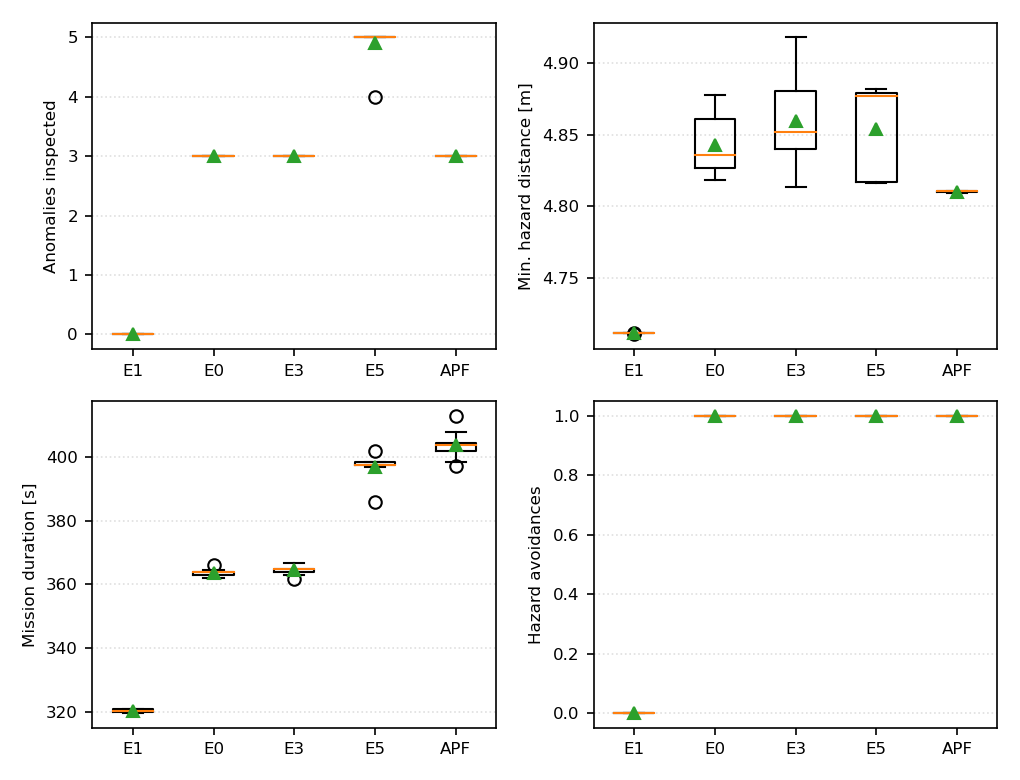
\includegraphics[width=\columnwidth]{box_panel}
\caption{Per-run distributions of the key metrics ($\triangle$ = mean) for the
fixed baseline (E1), the $\eta=0$ ablation (E0), the method (E3), the adverse
scenario (E5), and the potential-field baseline (APF). The fixed baseline never
inspects nor retreats; in the default scenario the affective configurations do so
consistently (tight boxes) with E0 matching E3, and APF matches inspection at a
longer mission duration. The dense adverse scenario (E5) shows a spread in
anomalies inspected---not every run completes all five---consistent with the
density limit reported in Section~\ref{sec:adverse}.}
\label{fig:box}
\end{figure}

\subsection{Detection and Inspection Behavior}
The central result is that the affective layer turns a coverage patrol into an
inspection behavior. The fixed baseline (E1) inspects \emph{no} anomalies: it
follows the round and never deviates ($0.0\pm0.0$). With \textsc{Stay Alert}, the
robot inspects \emph{all three} anomalies in every valid run of the default
scenario, at every setting of $\eta$ including the ablation $\eta=0$ (E0--E4 all
$3.0\pm0.0$; Cliff's $\delta=1$, exact permutation $p=1.1{\times}10^{-5}$ vs.\ E1);
this completeness degrades under high perception noise (Section~\ref{sec:robustness})
and dense clustering (Section~\ref{sec:adverse}), which we quantify honestly. The
artificial-potential-field baseline (APF) also inspects all three ($3.0\pm0.0$),
confirming that a comparably simple reactive scheme can produce the anomaly
response; the difference between the methods lies in efficiency and safety,
discussed below, not in raw inspection count. Fig.~\ref{fig:traj} shows the mechanism: the
affective layer leaves the patrol to reach each anomaly's standoff and returns,
whereas E1 traces the round directly.

\begin{figure}[t]
\centering
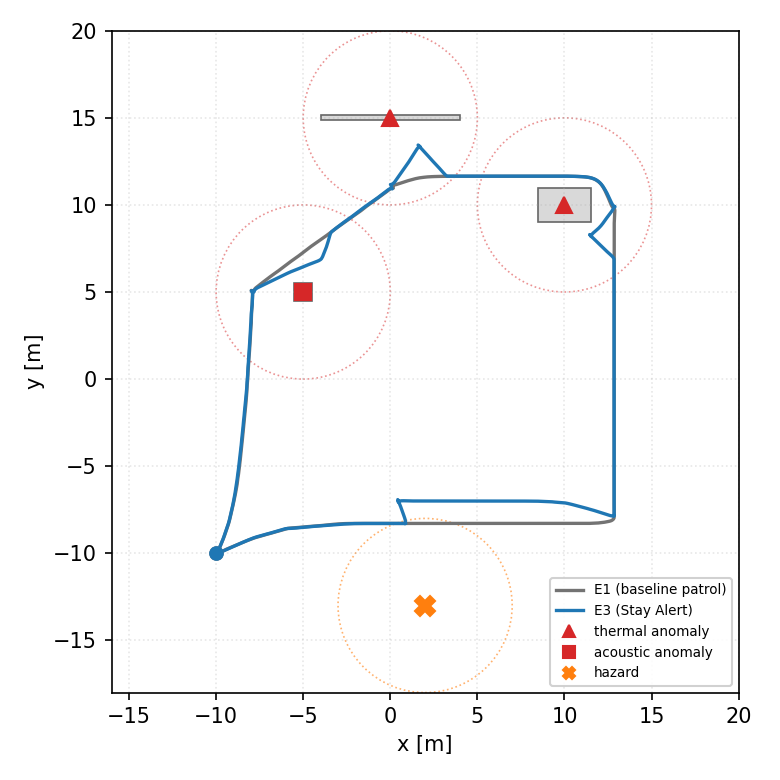
\includegraphics[width=\columnwidth]{traj_overlay}
\caption{Representative trajectories on the default scenario: the baseline
patrol (E1, gray) follows the round directly, whereas the proposed layer
(E3, Stay Alert, blue) deviates to approach the anomalies (thermal $\triangle$,
acoustic $\square$) and skirts the hazard ($\times$) zone. World frame, metres.}
\label{fig:traj}
\end{figure}

\subsection{Isolating the Field from the Act of Deviating}
\label{sec:heu}
%% R2#3: "the baselines fail to separate the affective weighting from a generic
%% same-controller heuristic". Esta subseção é a resposta. Dois contrastes:
%% HEU   = supervisor genérico completo (detecção bruta + seleção por proximidade)
%% HEUsel= UM fator (só o critério de seleção muda); tudo o mais igual ao método.
The comparisons above contrast the reactive layer with baselines that either cannot
deviate (the fixed patrol) or change the controller as well as the supervisor (the
potential-field baseline). Neither isolates the \emph{field} from the act of
deviating at all. We therefore add two configurations that run on the \emph{same}
Nav2/MPPI controller, with the same perception, keep-out, approach poses,
confirmation criterion and return-to-patrol logic:
\begin{itemize}
\item \textbf{HEU}, a generic detect--select--deviate--return supervisor: it is
triggered by \emph{raw detection} (an event inside the sensing radius) rather than by
a threshold on $\Phi$, selects the \emph{nearest} target rather than the most
salient, and arbitrates by the plain rule ``hazard in range $\Rightarrow$ deviate''.
It therefore discards both the saliency weighting and the categorical precedence.
\item \textbf{HEU-sel}, a one-factor variant: identical to the proposed layer
\emph{except} that it selects the nearest rather than the most salient target.
\end{itemize}
Changing the selected target does not alter $\Phi$ at the moment of triggering: the
simulator publishes the intensity of every event in range and the field retains the
maximum, so the threshold crossing is the same in both modes. It does, however, change
which anomaly is committed, and a committed anomaly stops feeding the field; the
contrast is thus one of selection at the decision point \emph{with} a downstream
effect on the time course of $\Phi$, not merely a reordering of service.

Table~\ref{tab:heu} reports the three scenarios. \textbf{Confirmatory (Holm-corrected
within the family declared in advance), \texttt{default} scenario:} HEU-sel is
indistinguishable from the proposed layer on every metric
($p_{\mathrm{Holm}}=1.0000$ throughout; $|\delta|\le0.19$; all bootstrap intervals
contain zero), whereas HEU differs in retreats ($1$ vs.\ $2$,
$p_{\mathrm{Holm}}=0.0034$), investigation time ($35.1$ vs.\ $41.2$~s,
$p_{\mathrm{Holm}}=0.0034$) and mission duration ($p_{\mathrm{Holm}}=0.0052$). The
clearance difference in this scenario does not survive correction
($p_{\mathrm{Holm}}=0.0511$) and amounts to $6$~cm, which we read as operationally
irrelevant and report as such rather than as an advantage.

\textbf{Exploratory, \texttt{conflict} scenario}---where a hazard is co-located with a
\emph{more salient} anomaly, so the two rules disagree by construction---the
difference is large and in the direction the precedence was designed to prevent. HEU
inspects the co-located anomaly (median $4$ of $4$ versus $3$ for the proposed layer)
and pays for it: minimum clearance falls from $4.84$ to $2.23$~m (Cliff's
$\delta=+1.00$, complete separation; bootstrap CI of the difference
$[+2.60,+2.63]$~m; $p<0.0001$), retreats rise from $1$ to $4$ as the supervisor
oscillates, mission duration grows by ${\approx}106$~s, and the time to inspect the
priority target is delayed by ${\approx}105$~s in both modalities
($345.0$ vs.\ $239.9$~s thermal; $387.6$ vs.\ $283.1$~s acoustic). HEU-sel again
matches the proposed layer on every metric.

\textbf{Exploratory, \texttt{adverse} scenario}: all three configurations inspect all
five anomalies; HEU performs one additional retreat and the clearance differences are
of the order of centimetres.

Two conclusions follow, and they point in opposite directions for the two components
of the field. The \emph{selection} rule is inert: replacing saliency by proximity
changed no measured outcome in any of the three scenarios. What is not inert is the
\emph{categorical precedence} carried by the sign of $\Phi$: discarding it, as the
generic supervisor does, trades safety and timeliness for one extra inspection
precisely when a hazard and a salient anomaly coincide. We therefore attribute the
reactive layer's advantage over a generic deviate-and-return heuristic to the
arbitration rule rather than to the saliency weighting, and we note that this is a
narrower claim than the one made in the previous version of this article.

\begin{table*}[t]
\centering
\caption{Proposed layer versus a generic detect--select--deviate--return supervisor
(HEU) and a one-factor selection variant (HEU-sel), all on the same Nav2/MPPI
controller. Medians over valid runs; $n$ per cell in the header. The
\texttt{default} row block is the confirmatory family (Holm-corrected); the
\texttt{conflict} and \texttt{adverse} blocks are exploratory and are reported with
uncorrected $p$.}
\label{tab:heu}
\footnotesize
\setlength{\tabcolsep}{4pt}
\begin{tabular}{llccccc}
\hline
\textbf{Scenario} & \textbf{Metric} & \textbf{Proposed} & \textbf{HEU} &
\textbf{HEU-sel} & \textbf{$\delta$ (vs.\ HEU)} & \textbf{$p$ (vs.\ HEU)}\\
\hline
\texttt{default} & Anomalies inspected        & $3$     & $3$     & $3$     & $+0.00$ & $1.0000^{\dagger}$\\
                 & Hazard retreats            & $1$     & $2$     & $1$     & $-1.00$ & $0.0034^{\dagger}$\\
                 & Min.\ hazard distance [m]  & $4.85$  & $4.91$  & $4.85$  & $-0.73$ & $0.0511^{\dagger}$\\
                 & Investigation time [s]     & $35.1$  & $41.2$  & $35.3$  & $-1.00$ & $0.0034^{\dagger}$\\
\hline
\texttt{conflict} & Anomalies inspected       & $3$     & $4$     & $3$     & $-0.67$ & $0.0160$\\
                 & Hazard retreats            & $1$     & $4$     & $1$     & $-1.00$ & $0.0003$\\
                 & \textbf{Min.\ hazard dist.\ [m]} & $\mathbf{4.84}$ & $\mathbf{2.23}$ & $4.82$ & $+1.00$ & $<\!0.0001$\\
                 & Mission duration [s]       & $363.7$ & $469.7$ & $364.4$ & $-0.89$ & $0.0013$\\
                 & Time to priority target [s]& $239.9$ & $345.0$ & $240.4$ & ---     & ---\\
\hline
\texttt{adverse} & Anomalies inspected        & $5$     & $5$     & $5$     & $-0.10$ & $0.7337$\\
                 & Hazard retreats            & $1$     & $2$     & $1$     & $-1.00$ & $0.0002$\\
                 & Min.\ hazard distance [m]  & $4.88$  & $4.90$  & $4.85$  & $-0.58$ & $0.0288$\\
\hline
\end{tabular}

\vspace{2pt}
\footnotesize $n$: \texttt{default} $10/9/10$, \texttt{conflict} $10/9/10$,
\texttt{adverse} $10/10/10$ (proposed/HEU/HEU-sel).
$^{\dagger}$Holm-corrected within the confirmatory family. Every
proposed-versus-HEU-sel comparison yields $p_{\mathrm{Holm}}=1.0000$ or
$p>0.22$ and is omitted from the last two columns for brevity.
\end{table*}

\subsection{Hazard Response and Safety}
The fixed baseline records zero hazard avoidances, while the affective layer
performs exactly one retreat per encounter ($1.0\pm0.0$). For the hazard placed
\emph{beside} the route (E0--E5), the minimum clearance is small in absolute
terms for both, but the affective layer keeps a slightly \emph{larger} and highly
consistent clearance (E3 $4.86\pm0.03$\,m) than the fixed baseline
($4.71\pm0.00$\,m): the repulsion regulates the approach to a tight band, and
the baseline---now that spawn-failure runs are separated out---passes the
beside-route hazard at a fixed, marginally closer distance. The more informative
test places the hazard \emph{on} a patrol leg (configurations RHM, the method,
and RHB, the fixed baseline). There, the fixed baseline drives straight through,
reaching a minimum clearance of only $0.71\pm0.00$\,m with no retreat and a
minimum time-to-collision of $2.8\pm0.1$\,s, whereas the affective layer produces
a two-timescale response: as soon as the hazard is detected it is projected as a
persistent keepout into the global costmap (so the planner routes around it for the
rest of the mission), and a fast reactive retreat ($1.0\pm0.0$ avoidance event)
handles the immediate proximity; the two together let the robot contour the hazard
at $1.71\pm0.01$\,m ($0$ collisions across valid runs) with a time-to-collision
margin of $5.6\pm0.9$\,s, while still inspecting all three anomalies ($3.0\pm0.0$),
at a time cost of $372\pm1$\,s. The
affective layer thus more than doubles the clearance
($+1.00$\,m; Cliff's $\delta=1$, $p<10^{-4}$) and roughly doubles the
time-to-collision margin ($+2.8$\,s; $p<10^{-4}$) of the fixed patrol on the case
the repulsion is meant to
handle---a hazard blocking the route---demonstrating the affective signal acting
on both the reactive and the deliberative layer (Table~\ref{tab:safety}).

\begin{table}[t]
\centering
\caption{On-route hazard: safety outcomes (mean\,$\pm$\,std over valid runs). RHB
is the fixed baseline (drives straight through); RHM is the method---a reactive
retreat combined with a detection-triggered persistent keepout that the planner
routes around. Valid $n$: RHB $10$, RHM $9$.}
\label{tab:safety}
\footnotesize
\begin{tabular}{lcc}
\hline
\textbf{Metric} & \textbf{RHB (baseline)} & \textbf{RHM (method)}\\
\hline
Anomalies inspected        & $0.0\pm0.0$   & $3.0\pm0.0$\\
Hazard retreats            & $0.0\pm0.0$   & $1.0\pm0.0$\\
Collisions                 & $0.0\pm0.0$   & $0.0\pm0.0$\\
Min.\ hazard distance [m]  & $0.71\pm0.00$ & $1.71\pm0.01$\\
Min.\ time-to-collision [s]& $2.8\pm0.1$   & $5.6\pm0.9$\\
Time below clearance [s]   & $14.4\pm0.0$  & $9.2\pm0.1$\\
Mission duration [s]       & $320\pm1$     & $372\pm1$\\
\hline
\end{tabular}
\end{table}

To attribute this safety gain to its two mechanisms, we ablate them
(Table~\ref{tab:ablation}). With the \emph{keepout alone} (KOa, reactive retreat
disabled) the planner still routes around the hazard and inspects all three
anomalies at the same $1.71$\,m clearance, slightly faster than the full method
($352$ vs.\ $372$\,s). With the \emph{reactive retreat alone} (KOb, keepout
disabled) the robot cannot clear the on-route hazard: it oscillates
($29.6\pm3.9$ retreats), inspects almost nothing ($0.2\pm0.4$), and times out
($627\pm6$\,s). %% R3#2: "A fairer reference for the safety claim is the fixed patrol plus the same
%% detection-triggered keepout, with no reactive layer at all." KOF e exatamente isso.
These two ablations still carry the reactive layer. Reviewer comment R3.2 asks for the
fairer reference: a \emph{fixed patrol carrying the same detection-triggered keep-out
and no reactive layer at all}. We therefore add configuration KOF (reactive layer
disabled, keep-out enabled). KOF reaches a median minimum clearance of $1.73$~m
against $1.71$~m for the keep-out-only ablation KOa---a difference of $2$~cm that is
not distinguishable ($p_{\mathrm{Holm}}=0.42$)---and spends $9.0$~s below the $2$~m
band against $9.3$~s. \textbf{We therefore attribute the safety benefit on an on-route
hazard to the detection-triggered keep-out, not to the reactive weighting}, and we
state this in the abstract and the conclusion rather than leaving the comparison
against a hazard-blind baseline to carry the claim.

What the reactive layer contributes over KOF is the inspection behavior itself, and
only that: KOF inspects $0$ of the $3$ anomalies in every run---by construction, since
with no reactive layer no investigation is ever triggered---against $3$ of $3$ for
KOa ($p_{\mathrm{Holm}}=0.0027$), and it completes the mission $31$~s faster
($320.9$ vs.\ $352.1$~s, $p_{\mathrm{Holm}}=0.0027$) precisely because it never
detours. The honest reading of the pair KOF/KOa is therefore a decomposition rather
than a victory: the keep-out buys the clearance, the reactive layer buys the
inspections, and they are separable.

The deliberative keepout is therefore the mechanism that resolves
an on-route hazard; the reactive retreat adds \emph{no} measurable benefit for this
\emph{static} hazard (KOa matches RHM and is slightly faster). We do not claim the
retreat helps here---its value instead appears when a hazard \emph{emerges} during
an investigation, which we quantify next (Section~\ref{sec:emerging}).

\begin{table}[t]
\centering
\caption{Keepout/retreat ablation on the on-route hazard (mean\,$\pm$\,std over
valid runs; $n=9$ for RHM, $10$ for KOa, $9$ for KOb). RHM is the full method
(retreat $+$ keepout); KOa is keepout-only (retreat disabled); KOb is retreat-only
(keepout disabled).}
\label{tab:ablation}
\footnotesize
\setlength{\tabcolsep}{5pt}
\begin{tabular}{lccc}
\hline
\textbf{Metric} & \textbf{RHM} & \textbf{KOa} & \textbf{KOb}\\
 & \textbf{(re.+ke.)} & \textbf{(keep.)} & \textbf{(retr.)}\\
\hline
Anomalies inspected        & $3.0\pm0.0$   & $3.0\pm0.0$   & $0.2\pm0.4$\\
Hazard retreats            & $1.0\pm0.0$   & $0.0\pm0.0$   & $29.6\pm3.9$\\
Collisions                 & $0.0\pm0.0$   & $0.0\pm0.0$   & $0.0\pm0.0$\\
Min.\ hazard distance [m]  & $1.71\pm0.01$ & $1.71\pm0.01$ & $4.29\pm0.08$\\
Min.\ time-to-collision [s]& $5.6\pm0.9$   & $5.8\pm0.1$   & $8.7\pm0.2$\\
Mission duration [s]       & $372\pm1$     & $352\pm1$     & $627\pm6$\\
\hline
\end{tabular}
\end{table}

\subsection{The Retreat's Value under an Emerging Hazard}
\label{sec:emerging}
The ablation above shows that, for a \emph{static} on-route hazard, the
deliberative keepout alone (KOa) matches the full method and the reactive retreat
adds no measurable benefit. The retreat is designed, however, for a hazard that
\emph{emerges} while the robot is already committed to an inspection---the case the
preemption of Algorithm~\ref{alg:stayalert} was built for and that the static
scenarios cannot exercise. We test this directly (configurations DHa, DHb): a
hazard co-located with an anomaly stays inactive---published to neither the
reactive channel nor the deliberative keepout---until the robot, already
investigating, closes to $3$~m, at which point the environment activates it (the
activation instant and the first publication to each channel are logged per run).
The clearance and radial time-to-collision values below are \emph{whole-mission}
minima relative to the hazard's location, including the pre-activation period: the
collector does not reset these metrics upon activation. These results therefore
compare overall mission-level margins in the emerging-hazard scenario and do not
estimate a separate post-activation TTC effect. The audit's preserved simulation
time does let us localize the \emph{distance} minimum: it is reached after
activation in all $18$ valid dynamic runs. We do \emph{not} extend this to the TTC
minimum---which, being a ratio involving radial speed, can already carry a
pre-activation value (in one run the final TTC minimum is recorded just before
activation)---so the TTC difference is reported strictly as a whole-mission margin. With the
reactive retreat enabled (DHa) the preemption fires in \emph{every valid run}
($8/8$ deferred investigations) and the robot backs off, keeping a minimum
clearance of $2.55\pm0.15$\,m and a radial time-to-collision of $5.23\pm0.45$\,s.
With the retreat disabled (DHb, keepout only) the robot instead proceeds to the
inspection standoff, closing to $2.22\pm0.01$\,m ($4.72\pm0.21$\,s). The reactive
retreat therefore buys $+0.33$\,m of clearance ($95\%$ CI $[+0.23,+0.42]$, Cliff's
$\delta=1$, $p=4.6{\times}10^{-5}$) and $+0.51$\,s of time-to-collision margin
($[+0.20,+0.84]$, $\delta=0.85$, $p=1.0{\times}10^{-3}$) against an emerging
hazard. This margin is a deliberate trade, not a free gain: DHa runs about
$9.4$~s longer ($348$ vs.\ $338$~s) and $1.6$~m farther, and \emph{defers} the
now-hazardous inspection (DHa inspects the target in no run; DHb in every run),
buying a larger safety margin at that encounter at the price of a completed
inspection. Neither configuration enters the contact region, and neither spends
any time below the $2$~m clearance threshold, so the effect is a difference in
\emph{margin}, not in observed contacts. We also distinguish the preemption
firing from a cleanly completed retreat: in $3$ of the $8$ valid DHa runs the
retreat's navigation goal is itself aborted, yet each episode still ends as a
successful avoid---the field decays below threshold once the hazard is handed to
the keepout (\emph{safe} exit)---and the clearance we report is the
\emph{true-position} minimum from the metrics collector, not an assumed arrival at
the retreat pose (those three runs in fact hold $2.70$~m). The retreat's
contribution is thus a \emph{transient} safety margin when a hazard appears
mid-investigation---a benefit the static on-route ablation, by construction,
cannot reveal.

\subsection{Safety Precedence under Conflict}
\label{sec:conflict}
The preceding scenarios separate attraction and repulsion in space, so the field
never has to arbitrate between an anomaly and a hazard at the same location. The
conflict scenario (CONF) forces exactly that decision: a \emph{strong} acoustic
anomaly ($|w\,I_e|=1.14$) is co-located with a \emph{weaker} hazard
($|w\,I_e|=1.05$) at $(2,-13)$, so a magnitude-only selection rule---which keeps
the more salient signal---would prefer to inspect the anomaly and never trigger
a retreat. The precedence rule of Eq.~\eqref{eq:phi-update} instead resolves any
above-threshold hazard first, independently of a concurrent, stronger attraction.
This is a categorical \emph{selection} property, not an average effect, so we
report it as an outcome frequency rather than a mean comparison. Across all ten runs of CONF
(all valid), the behavior was identical in every run: \textsc{Avoid} was
triggered ($10/10$ runs, $1.0\pm0.0$ retreats) and the co-located strong anomaly
was \emph{never} inspected, so the robot inspected only the three off-conflict
anomalies ($3.0\pm0.0$; the fourth event is the co-located pair). The robot kept a
minimum hazard clearance of $4.84\pm0.02$\,m and a minimum time-to-collision of
$17.3\pm1.6$\,s, with \emph{zero} collisions across all runs, at a mission duration
($364\pm2$\,s) indistinguishable from the default scenario. The affective
field therefore enforces a \emph{hazard-first selection priority} by construction,
confirmed empirically in the one case designed to break a magnitude-only
interpretation. This is a deliberate design choice---the priority is \emph{hard},
so a hazard barely above threshold (a potential false positive) suppresses even a
strongly salient genuine anomaly---and we accept the resulting risk of
over-conservatism near the threshold. We distinguish this \emph{logical} priority
from a physical safety guarantee: it holds under explicit conditions (an available
retreat pose, and outside the post-retreat refractory window), and the static CONF
scenario does not exercise cases such as a second hazard appearing during the
refractory; what we report as a safety \emph{outcome} is the observed clearance and
the absence of contact-region entries, not an invariance guarantee.

\subsection{The Cost of the Precedence, and Its Sensitivity}
\label{sec:precedence-cost}
%% R2#6: "A hazard barely above threshold suppresses even a strongly salient genuine
%% anomaly, and the authors acknowledge the resulting over-conservatism risk. A
%% sensitivity analysis around the hazard threshold, or a scenario with a marginal
%% hazard and a high-value inspection target, would strengthen the claim that the
%% precedence is not merely correct-by-construction but also operationally sensible."
%% Fazemos as duas coisas. Exploratorio.
The preceding subsection accepts a risk of over-conservatism near the threshold
without measuring it. We now measure it, and separately probe whether the threshold
that governs the precedence is well placed. Both analyses are exploratory.

\paragraph*{A marginally eligible hazard costs one inspection, deterministically}
The hazard channel has memory: an observation raises $h$, and $h$ then decays by
$\lambda$ per period until it falls below $\varepsilon$. Because the modality
threshold is applied to the raw perceived intensity, the \emph{weakest} eligible
hazard already yields $h=|w_{\mathcal{H}}|\,\theta_{\mathcal{H}}$, which here equals
the supervisor's entry threshold; a retreat therefore fires once, at the peak. After
a single decay step, however, $h$ is below the entry threshold while still above
$\varepsilon$---so the hazard keeps \emph{governing} the field, and thus keeps
suppressing any attraction, without triggering any further retreat. We built
configuration CM to exercise exactly this band: a hazard of minimal eligible
intensity beside the first patrol leg, which the robot observes and then leaves
behind, together with a legitimate acoustic anomaly of intensity $0.95$---the most
salient event in the scenario---placed $4.3$~m from the hazard, well outside it.

The result is deterministic across all ten runs. The suppression window lasts
$69.5$~s (range $67.3$--$72.4$), exactly one retreat fires, and the salient anomaly
is \emph{never} inspected: $0/10$ runs, so the robot ends every mission having
inspected $3$ of the $4$ anomalies, and the one it forfeits is the strongest. The
priority-target metric records the same outcome from the other side: the acoustic
priority target is censored at the $400$~s horizon in $10/10$ runs. The categorical
precedence therefore does not merely risk over-conservatism---in this configuration
it costs one inspection in every run, and the cost is incurred while the robot is in
no danger, since the hazard is by then too weak to warrant retreating from.

We emphasise one reading that the numbers do not support. CM and the full conflict
scenario both end with three anomalies inspected, but the two threes are not
comparable: in CONF the forfeited anomaly is co-located with the hazard and
\emph{should} be refused, whereas in CM it is a legitimate target $4.3$~m away. The
same count is correct behavior in one scenario and a failure in the other.

\paragraph*{The threshold governing the precedence is well placed, and raising it
costs clearance} Varying the supervisor's entry threshold does not test the
precedence, because what governs suppression is the \emph{modality eligibility}
threshold $\theta_{\mathcal{H}}$ applied before weighting. We sweep that threshold
over $\{0.20,0.30,0.40\}$ in the conflict scenario, with $0.30$ the value used
throughout. Lowering it to $0.20$ changes nothing measurable (clearance $4.85$ vs.\
$4.83$~m, $p=0.39$; identical inspections and retreats). Raising it to $0.40$
\emph{degrades} safety: the minimum clearance falls to $3.78$~m (Cliff's
$\delta=+1.00$, bootstrap CI of the difference $[+0.99,+1.10]$~m, $p<0.0001$) and the
mission lengthens by $9.1$~s, because a higher eligibility threshold means the hazard
is recognised later and therefore closer. The sweep thus yields a conclusion rather
than a range: the operating point is at a plateau on one side and a cliff on the
other, and the clearance reported elsewhere in this article is not an artifact of a
conveniently chosen threshold.

\paragraph*{Hysteresis: width is immaterial, position is not}
%% R3#3 pede os valores de histerese e limiar como sensibilidade. Os tres pares
%% separam POSICAO de LARGURA -- um par que mude as duas coisas nao permitiria
%% atribuir o efeito.
We compare three entry/exit pairs chosen so that position and width vary
independently: the reference $(0.45,0.25)$ of width $0.20$; a narrower band
$(0.45,0.35)$ of width $0.10$ at the same entry point; and a shifted band
$(0.55,0.35)$ of the same width $0.20$. Halving the width changes nothing: route
deviations, inspections, mission duration and investigation time are all
indistinguishable from the reference ($p\ge0.60$). Shifting the entry point doubles
the counted route deviations ($4\rightarrow8$, $\delta=-1.00$, $p=0.0003$) and
shortens the mean investigation episode ($35.1\rightarrow26.6$~s, $p=0.0003$), while
leaving the inspections unchanged at $3$ of $3$: with a higher entry threshold the
robot lingers longer in the aroused-but-uncommitted band and commits closer to the
target. The behavior of interest is therefore robust to the hysteresis width, and the
\texttt{route deviations} metric should be read as sensitive to the \emph{position}
of the entry threshold rather than as a scenario-intrinsic count.

\subsection{Cost of the Inspection Behavior}
The added behavior is inexpensive: the mission duration of E3 ($364\pm1$\,s) is a
modest increase over the fixed baseline ($320\pm1$\,s) for the inspection
detours ($+6.2$\,m travelled). Framed as a utility trade-off, each additional
anomaly inspected costs about $2$\,m of extra travel ($+6.2$\,m for three) and
$15$\,s of mission time ($+44$\,s for three)---a favorable exchange given that
the fixed baseline inspects \emph{none}.

%% R3#3 pede a comparacao com o APF consolidada numa tabela unica, com intervalos,
%% e a declaracao do procedimento e do ESFORCO de ajuste. Tambem corrigimos aqui a
%% afirmacao da versao anterior de que o baseline de mesmo controlador ficava como
%% trabalho futuro: ele agora existe (Secao~\ref{sec:heu}).
Table~\ref{tab:apf} consolidates the comparison against the potential-field
baseline, which the previous version of this article reported across several tables.
The proposed layer completes the same three inspections faster ($364$ vs.\
$404\pm5$\,s). We are explicit about what this does \emph{not} isolate: the APF
baseline replaces the reactive supervisor \emph{and} the controller---it commands
velocities directly instead of issuing Nav2/MPPI goals---so the difference confounds
the supervisor with the controller. On tuning effort we are equally explicit: the APF
gains were set by manual sweep until the baseline completed the default scenario
without local-minimum stalls, and its approach parameters differ from ours (standoff
$1.8$~m and a $30$~s investigation budget, against $2$~m and $40$~s;
Table~\ref{tab:hyper}). We did not invest comparable effort in tuning the baseline's
thresholds to those of the proposed layer, and the time advantage should be read with
that asymmetry in mind. The comparison that \emph{does} isolate the supervisor, on a
shared controller and shared parameters, is the heuristic of Section~\ref{sec:heu};
the earlier version of this article left that baseline as future work and it is now
part of the study.

\begin{table}[t]
\centering
\caption{Consolidated comparison against the potential-field baseline (default
scenario, valid runs; $n=10$ proposed, $n=9$ APF). Mean\,$\pm$\,std, with the $95\%$
bootstrap interval of the difference. The two configurations differ in both
supervisor and controller, so the difference is not attributable to the reactive
layer alone.}
\label{tab:apf}
\footnotesize
\setlength{\tabcolsep}{4pt}
\begin{tabular}{lccc}
\hline
\textbf{Metric} & \textbf{Proposed (E3)} & \textbf{APF} & \textbf{$95\%$ CI of diff.}\\
\hline
Anomalies inspected        & $3.0\pm0.0$   & $3.0\pm0.0$   & $[+0.00,+0.00]$\\
Mission duration [s]       & $364\pm1$     & $404\pm5$     & $[-43.1,-36.8]$\\
Distance travelled [m]     & $86.6\pm0.2$  & $88.9\pm1.1$  & $[-3.1,-1.6]$\\
Min.\ hazard distance [m]  & $4.86\pm0.03$ & $4.79\pm0.06$ & $[+0.03,+0.11]$\\
Time to priority target [s]& $240.8$       & $269.7$       & $[-34.2,-23.1]$\\
\hline
\end{tabular}
\end{table}

\subsection{Adverse Scenario}
\label{sec:adverse}
In the event-dense scenario (E5) the robot arbitrates between clustered events by
the precedence rule of Eq.~\eqref{eq:phi-update}, inspecting on average
$4.9\pm0.3$ of the five anomalies with correspondingly more deviations
($9.4\pm0.8$) and a longer mission ($397\pm4$\,s). Full inspection of all five
succeeds in $9$ of $10$ runs ($95\%$ Wilson interval $[0.60,0.98]$). The
per-episode audit trail (Section~\ref{sec:setup}) shows the cause precisely: all
five targets are \emph{started} in every run, and the incompleteness is a
navigation failure, not a failure to revisit. Three runs recorded a reactive
navigation failure; two of them subsequently \emph{started an additional
investigation} and completed all five targets, while the remaining run ended with
four credited inspections and \emph{no further recorded attempt} on the failed
target. The two additional investigations are reported as an observation of the
episodes, not as a demonstrated retry policy: the \texttt{failed} branch marks the
target as failed but does not remove it from the committed set, so a later start is
possible but not guaranteed by an explicit recovery rule. This density limit---the
reactive navigation occasionally failing on a tightly clustered target---is measured
honestly here rather than assumed away, with no contact-region entries observed
(zero collisions). We do not claim general scaling from a single adverse
configuration, and broader density and geometry sweeps remain future work.

%% R3#1 (reposicionamento editorial): a subseção 'Value-Function Stability' e a
%% Fig. do resíduo foram movidas para o Apêndice~\ref{app:update} junto com a
%% formulação. Elas atestam que o update é estável, não que ele governe
%% comportamento -- manter no corpo dava-lhes um peso que o resultado não sustenta.

\subsection{Robustness to Perception Noise}
\label{sec:robustness}
Because the event abstraction supplies modality, intensity, and position without
uncertainty, we probe the method's sensitivity to this idealization by injecting
zero-mean Gaussian noise on the perceived event position and intensity at each
sensing tick. Under moderate noise (position $\sigma=0.3$\,m, intensity
$\sigma=0.05$; configuration N1) the method is unaffected: it inspects all three
anomalies in every valid run ($3.0\pm0.0$), with the hazard response preserved and
no collisions. Under high noise ($\sigma=0.6$\,m, $\sigma=0.10$; N2), inspection
completeness degrades to $4/9$ full inspections, and the run logs let us attribute
the cause precisely: all three anomalies are still \emph{detected} in every run, but
the noisy position estimate steers the robot to a point from which the evaluator
cannot confirm arrival at the \emph{true} anomaly, so $6$ of the $27$ committed
inspections (across the $9$ valid runs) are \emph{confirmation rejections}---not
navigation timeouts or aborts, of which the CSVs record none. Full inspection
therefore succeeds in $4$ of $9$ valid runs ($2.3\pm0.7$ anomalies; $95\%$ Wilson
interval $[0.19,0.73]$ for the per-mission completion rate). No contact-region
entries were observed, and the hazard retreat was preserved ($1.7\pm0.5$;
Table~\ref{tab:noise}); the mean minimum hazard clearance in fact \emph{increased}
from $4.86\pm0.03$\,m in E3 to $5.29\pm0.20$\,m in N2. These results describe the
observed trade-off under the tested noise levels---inspection completeness falls
(through the confirmation step) while no contacts are observed and the measured
clearance grows---and do not establish a general safety guarantee. We report per-mission completion with its Wilson
interval rather than treating the three anomalies of a run as independent trials.

\begin{table}[t]
\centering
\caption{Robustness to perception noise (method, mean\,$\pm$\,std). E3 is
noiseless; N1 and N2 add moderate and high zero-mean Gaussian noise on event
position ($\sigma_p$) and intensity ($\sigma_i$). ``Full-inspection rate'' is the
per-mission fraction of runs inspecting all three anomalies (with the confirmed
arrival of Section~\ref{sec:results}); safety (collisions, clearance) is
maintained across all noise levels. Valid $n$: E3 $10$, N1 $10$, N2 $9$.}
\label{tab:noise}
\footnotesize
\begin{tabular}{lccc}
\hline
\textbf{Metric} & \textbf{E3 (none)} &
\textbf{N1 ($\sigma_p{=}0.3$)} & \textbf{N2 ($\sigma_p{=}0.6$)}\\
\hline
Anomalies inspected       & $3.0\pm0.0$  & $3.0\pm0.0$  & $2.3\pm0.7$\\
Full-inspection rate      & $10/10$      & $10/10$      & $4/9$\\
Hazard retreats           & $1.0\pm0.0$  & $1.1\pm0.3$  & $1.7\pm0.5$\\
Collisions                & $0.0\pm0.0$  & $0.0\pm0.0$  & $0.0\pm0.0$\\
Min.\ hazard distance [m] & $4.86\pm0.03$& $5.01\pm0.11$& $5.29\pm0.20$\\
Mission duration [s]      & $364\pm1$    & $367\pm5$    & $374\pm8$\\
\hline
\end{tabular}
\end{table}

\paragraph*{Is the degradation a property of the method or of the confirmation
criterion?}
%% R2#5: "if the confirmation distance is 3.3 m and the noisy position estimate
%% steers the robot away from the true anomaly, is the reported degradation a
%% property of the method or of the confirmation criterion? A sensitivity analysis
%% over the confirmation distance would help disentangle these."
%% O criterio e uma funcao de PONTUACAO pura: nao realimenta o comportamento (a
%% supressao de re-atracao depende de 'committed', marcado no inicio do episodio, e
%% a nao-confirmacao nao o libera). Logo a varredura e RETROSPECTIVA, sobre as
%% MESMAS trajetorias, sem executar nada de novo.
An inspection is credited only if the robot is within a confirmation distance of the
\emph{true} event position when the episode closes; we use $3.3$~m. This criterion
scores the outcome and does not feed back into the controller---the suppression of
re-attraction keys on the target being committed at the \emph{start} of an episode,
and a non-confirmation does not release it---so the same recorded trajectories can be
re-scored under other thresholds without executing anything new. We do so
retrospectively, and label it as such.

Re-scoring reproduces the published figure exactly at $3.3$~m ($4/9$ full inspections
under high noise), which validates the procedure. It also shows the reported
completeness to be strongly criterion-dependent: at $2.8$~m the high-noise rate falls
to $2/9$, and at $4.0$~m it recovers to $9/9$. The robot did approach the anomalies;
under high noise it stopped $2.9$--$3.6$~m away because the perturbed position
estimate displaced the inspection pose, and the $3.3$~m criterion then refused those
approaches. That is only half the answer, however, because the physical approach also
degrades: the distance to the true target at episode close rises from $2.23$~m
(median, range $2.21$--$2.24$) with clean perception to $2.87$~m (range
$1.83$--$3.56$) under high noise. Both effects are present and we report them
together; the defensible statement is that \emph{the completeness figure is sensitive
to the confirmation criterion and the approach quality genuinely degrades}, not that
the degradation is an artifact. We note the measured quantity is the distance at
episode close, not the minimum over the approach, which is not instrumented per run.

\paragraph*{Does the discontinuity at $d=R$ affect the state machine?}
%% R2#8: "the profile still produces an intensity of Ie/2 at the boundary and zero
%% immediately beyond, which is a discontinuity in the reported signal. A brief
%% statement of whether this discontinuity has any measurable effect on the FSM
%% transitions would be useful."
%% Uma contagem global de transicoes nao identificaria o efeito da fronteira, e uma
%% trajetoria tangente poderia so tocá-la. A ronda real cruza d=R nos dois sentidos
%% varias vezes por run, entao medimos sobre os logs existentes.
The intensity profile is $I_e/2$ at $d=R$ and zero immediately beyond, a step in the
reported signal. The patrol crosses this boundary in both directions several times
per run, so we measure its effect on the existing logs rather than constructing a
dedicated trajectory---a tangential path risks touching the boundary without crossing
it. Taking a gap in the field trace as time spent outside every sensing radius, the
first sample after a gap is an inward crossing and the last before it an outward one.
Across the default scenario we observe $30$ inward and $30$ outward crossings in ten
runs, with a median jump at entry of $0.436$ (maximum $0.686$), consistent with the
$|w\,I_e/2|$ predicted by the profile: the discontinuity is real and of the expected
size. Only $10$ of those $30$ inward crossings are followed by a state transition
within $2$~s, so the step does not reliably drive the machine. The shortest interval
between consecutive transitions is $9.8$~s in the default scenario and $7.0$--$9.6$~s
in the noise and conflict scenarios, with no sign of boundary chattering. In the
dense scenario the shortest interval is $0.2$~s, and inspection of those cases shows
they are not threshold oscillation: they are either back-to-back servicing of a
cluster---one anomaly credited and the next, already well inside range at
$\Phi\approx0.5$, committed immediately---or an episode ended at once by a transient
Nav2 goal abort. Neither arises from the boundary.

\subsection{Threats to Validity}
The evaluation is in simulation; field behavior may differ. The
sensing-and-perception chain is abstracted as events, so the inspection rate
measures the \emph{navigation-and-decision} response, not perception accuracy;
we probe sensitivity to this abstraction with the perception-noise sweep
(Section~\ref{sec:robustness}), which also exposes the method's limits: inspection
completeness degrades under high perception noise ($4/9$) and dense clustering
($9/10$) (measured, not assumed), while no contact-region entries were observed in
any scenario. The safety metrics are
proxies computed from the \emph{true} hazard position and should be read as such:
``collisions'' counts entries into a simulated contact region (centre-to-centre
distance below $0.5$~m), not readings of a physical contact sensor, and
``time-to-collision'' is a radial-closing proxy ($d/\dot d$ to the nearest hazard),
not the trajectory-intersection time with a finite hazard region; zero collisions
in a group bounds but does not eliminate risk (the \emph{exact} one-sided $95\%$
binomial bound on the failure probability for zero observed failures,
$1-0.05^{1/n}$, is $\approx26\%$ for a $10$-run group, $\approx28\%$ for a
$9$-run group, and $\approx31\%$ for the $8$-run DHa group; this risk bound is
distinct from the Wilson-score intervals used for the descriptive success rates).
%% R3-m2: "Please give the per-configuration counts in the main text next to the
%% headline numbers, since results such as 4/9 depend on them, and note whether the
%% exclusion could favor any configuration." A segunda parte e a desconfortavel.
A fraction of runs ($6$ of $160$ in the earlier battery, $3$ of $130$ in the new
one) remained immobile (travelled distance $\approx0$); these are reported
separately as a startup-reliability outcome and excluded from the behavioral
statistics. The valid counts are $n=10$ for every configuration except APF, KOb, N2
and RHM ($n=9$), DHa ($n=8$), and the two new heuristic blocks in the
\texttt{default} and \texttt{conflict} scenarios ($n=9$); every rate in this article
is reported against its own denominator, which is why the high-noise completeness
reads $4/9$ and the dense-clustering completeness $9/10$.

Whether the exclusion can favor a configuration deserves a direct answer rather than
an assumption of independence, and the answer differs by metric. All excluded runs
inspected zero anomalies, so removing them \emph{raises} every completeness figure;
for the pair most affected it raises the proposed layer and the APF baseline by the
same amount ($2.7\rightarrow3.0$ anomalies each), leaving their difference unchanged
but making both absolute figures conditional on successful initialization. For
safety the adjustment runs the other way: a run in which the robot never moved
trivially records zero contact-region entries, so including such runs would inflate
the evidence for contact-free navigation, and they are therefore excluded from the
safety statistics as well. We do not claim that start-up failure is independent of
configuration---the exclusions are not uniformly distributed across blocks---only
that the direction of each adjustment is stated and that both views are reported. Event identity and inspection pose are published on
separate topics within the same sensing tick rather than as one timestamped
message; for the single-salient-target dynamics evaluated here they refer to the
same observation, but guaranteeing this under rapid target switching is left as an
implementation refinement. Localization is idealized---the
map$\rightarrow$odom transform is held fixed---so localization drift is not modeled
(Section~\ref{sec:setup-repro}). The value function is tabular, and the
value-update formulation is a design note (Appendix~\ref{app:update}) rather than
the mechanism controlling the robot here. These
choices are documented for reproducibility (Section~\ref{sec:setup-repro}).

%% R2-Q3: "the limitations section is candid, but several acknowledged gaps are
%% stated rather than probed". Tres delas passaram a ser medidas nesta versao.
Three gaps that earlier versions of this article acknowledged without probing are now
measured, and we point to the measurements rather than repeating the acknowledgement.
The risk of over-conservatism near the hazard threshold is quantified in
Section~\ref{sec:precedence-cost}, where a marginally eligible hazard is shown to
cost one inspection in every run; the sensitivity of the reported completeness to the
confirmation criterion is quantified by re-scoring the same trajectories at other
thresholds; and the claim that the reactive layer outperforms a generic
deviate-and-return behavior is now tested directly against such a behavior on the
same controller (Section~\ref{sec:heu}), with the result that the saliency weighting
is inert and only the arbitration survives. The gaps that remain stated rather than
probed are those requiring a different perception model: false positives and
negatives, event persistence, and localization drift.

\paragraph*{Provenance of the field signal} For auditability we note that the value
of $\Phi$ written into the value update is sampled in the odometry callback, whereas
the value published to the reactive supervisor is sampled by a $1$~Hz timer. Both
read the same field object, so they differ only in sampling instant; this does not
affect the executed behavior, which is driven by the published signal, but it means
the two series in the released logs are not sample-aligned.
